\section{Notaciones y definiciones}

Comencemos revisando la notación matemática que se utilizará en este libro, así como algunas definiciones y teoremas que nos serán de utilidad en el desarrollo de los temas.

\begin{definition}
    Escalar 

    Un escalar es un número perteneciente a los conjuntos $\R$  o $\C$. Una forma elegante
    de llamar a los números.
    Cuando se hable de un escalar, se asumirá que se está hablando de un número real, a menos que se 
    especifique lo contrario y se lo notará en itálica.
\end{definition}


\begin{definition}
    Lista 

    Supongamos $n$ es un número positivo. Una lista de longitud $n$ es una colección ordenada de $n$ elementos 
    (que pueden ser escalares, vectores o cualquier entidad matemática) rodeados por paréntesis y separados por comas.
    Una lista de longitud $n$ se ve de la siguiente forma:
    \begin{equation}
        (x_1, x_2, \ldots, x_n)
    \end{equation}

    Además dos listas son iguales si y solo si sus elementos correspondientes son iguales.
\end{definition}

\begin{definition}
    $\K^n$
    
    Si consideramos $\K$ como $\R$ o $\C$ entonces $\K^n$ es el conjunto de todas las listas de longitud $n$ de elementos de $\K$.
    $ \K^n = \{(x_1, x_2, \ldots, x_n) \,|\, x_i \in \mathbb{K}, \forall i = 1, 2, \ldots, n\}$.
\end{definition}

\begin{definition}
    Vector
    
    Un vector es un elemento de un espacio vectorial. Como no vamos a definir espacios vectoriales en este libro, un vector simplemente es una lista de números reales o complejos. Un vector de longitud $n$ es un elemento de $\mathbb{K}^n$. Los denotaremos con letras minúsculas en negrita. Y usaremos la notación $\mathbf{x}_i$ para referirnos al $i$-ésimo elemento de un vector.
\end{definition}

Los vectores pueden ser visualizados como puntos o flechas en un espacio $n$-dimensional.

\begin{figure}[htbp]
    \centering
    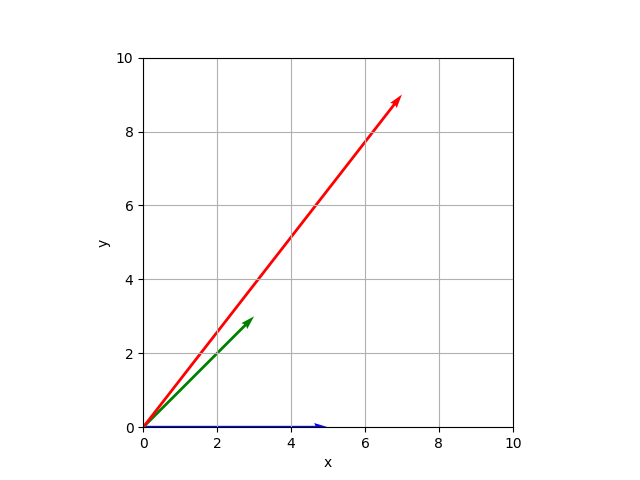
\includegraphics[width=0.4\textwidth]{Images/1/vectors.png}
    \hspace{2cm} 
    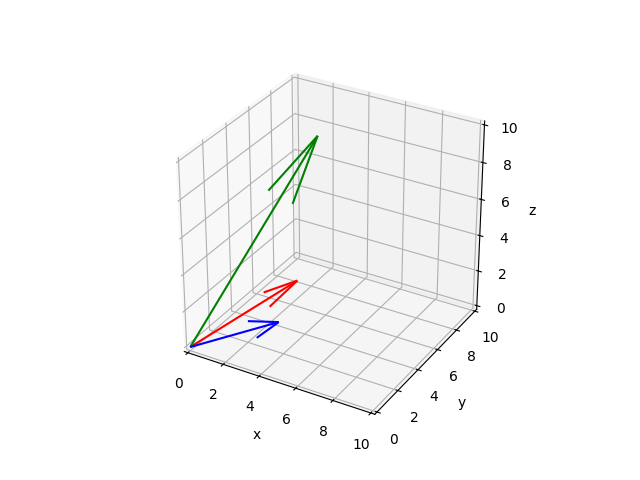
\includegraphics[width=0.4\textwidth]{Images/1/vectors_3d.png}
    \caption{Visualización de vectores en $\R^2$ y $\R^3$ respectivamente.}
    \label{fig:imagenes}
\end{figure}

\lipsum[1]

\begin{theorem}
    Here goes a theorem.
    \lipsum[1]
\end{theorem}

\begin{proof}
        Here goes the proof

    \lipsum[2]
\end{proof}


\begin{corollary}
    Here goes a corollary
\end{corollary}

\begin{eg}
    Here goes an example
\end{eg}

\begin{note}
    Here goes a note 

    \lipsum[2]
\end{note}


\begin{lemma}
    Here goes a lemma
\end{lemma}

\begin{prop}
    Here goes a proposition
\end{prop}

\subsection{Examples 2}
